\subsubsection{\stid{2.06} Exa-PAPI}\label{subsubsect:exapapi}

\paragraph{Overview} 

The Exascale Performance Application Programming Interface (Exa-PAPI) project
builds on the widely deployed and widely used Performance API (PAPI) and
extends it with performance counter monitoring capabilities for new and
advanced ECP hardware and software technologies, fine-grained power management
support, and functionality for performance counter analysis at task granularity
for task-based runtime systems. Exa-PAPI also adds events that originate from
the ECP software stack (i.e., communication libraries, math libraries, task
runtime systems, etc.) and, as a result, extends the notion of performance
events from strictly hardware-related ones to include software-based information. 

Exa-PAPI is essential for ECP because it enables the ECP application community
to monitor both types of performance events---hardware- and
software-related---in a uniform way, through one consistent PAPI interface. On
the hardware side, Exa-PAPI provides access to a wide range of new
events for the extreme-scale platforms that will form the basis of exascale
computing. Furthermore, it provides a finer-grain measurement and control of
power, thus offering software developers a basic building block for dynamic
application optimization under power constraint.  In addition to providing
hardware counter based information, Exa-PAPI integrates a standardizing layer
for monitoring software-defined events (SDEs), which will expose the internal behavior
of runtime systems and libraries to the applications. Addressing the gap of
software-defined event monitoring---and enabling monitoring of both types of
performance events though Exa-PAPI---stands to offer a transformative impact on
performance analysis and application development as a whole.


\paragraph{Key Challenges}

Widely deployed and widely used, PAPI has established itself as fundamental
software infrastructure in every application domain where improving performance
can be mission critical. 
However, processor and system designs have been experiencing radical changes.
Systems now combine multi-core CPUs and accelerators, shared and
distributed memory, PCI-express and other interconnects, and
power efficiency is emerging as a primary design constraint.
These changes pose new challenges and bring new
opportunities to PAPI. At the same time, the ever-increasing importance of
communication and synchronization costs in parallel applications, as well as the
emergence of task-based programming paradigms, pose
challenges to the development of performance-critical applications and create a
need for standardizing performance events that originate from various ECP
software layers.


\paragraph{Solution Strategy}

The Exa-PAPI project prepares the PAPI library to stand up to the challenges posed 
by exascale systems by:
(1) widening its applicability and providing robust support for hardware resources that 
are currently out of PAPI's scope;
(2) supporting new programming paradigms, such as task-based systems, by adding 
functionality for performance counter analysis at task granularity (as opposed to core 
and thread granularity); 
(3) extending PAPI to support software-defined events, in addition to the traditional 
hardware-based events; and 
(4) applying semantic analysis to hardware counters so that the application developer 
can better make sense of the ever-growing list of raw hardware performance events 
that can be measured during execution.

The Exa-PAPI effort delivers new PAPI components to handle the wide range of
new hardware and software events for the extreme scale platforms that will form
the basis of exascale computing. To achieve this, Exa-PAPI implements a variety
of monitoring and sampling capabilities for the different technologies, which
are exported to the ECP application community. 
%
Exa-PAPI also provides finer-grain measurement and control of power, thus
offering software developers a basic building block for dynamic application
optimization under power constraint. Other hardware efforts in Exa-PAPI are the
development of components for monitoring network interconnect events, as well as
components targeted at the deep and heterogeneous memory hierarchies that we
are already seeing in new architectures.


\paragraph{Recent Progress}

On the \textbf{software event} front, we began with the design and implementation of a new API to 
expose any kind of software-defined events. It extend PAPI�s role so that it becomes 
the de-facto standard for exposing performance-critical events from different software
layers.

%Because the PAPI SDE API will be used by different ECP libraries, and runtimes, 
%and also applications, this has been a Co-Design effort, and we have 
%shared our early Prototype API version with the community to gather feedback from the 
%different ECP teams.
%These interactions revealed two principal concerns. First, performance analysis tools 
%community strongly emphasized the importance of preserving the existing API,
%which is currently exported by PAPI for measuring hardware events.
%Second, library and runtime communities were mostly concerned with the performance 
%overhead caused by the introduction of SDEs in their codes.
%
%Since PAPI is positioned as a middleware layer, success depends on adoption 
%by other software modules and toolkits. As a result, we used the feedback from  
%the different communities to guide our design decisions.

Since the concept of software-defined events is new to PAPI, we worked closely with 
developers of different libraries and runtimes that serve as natural targets for early 
adoption of the new SDE API.
As of today, we have integrated SDEs into the sparse linear algebra library MAGMA-Sparse 
(2.3.3.10 STMS11-PEEKS), the tensor algebra library TAMM (2.2.1.02 ADSE11-NWChemEx), 
the task-scheduling runtime PaRSEC (2.3.1.09 STPM11-ParSEC), and the compiler-based 
performance analysis tool BYFL (HT-DSE). 

\vspace{-4pt}
\begin{figure}[!h]
\begin{center}
  \subfloat[ ]{\label{fig:sde_magma}
  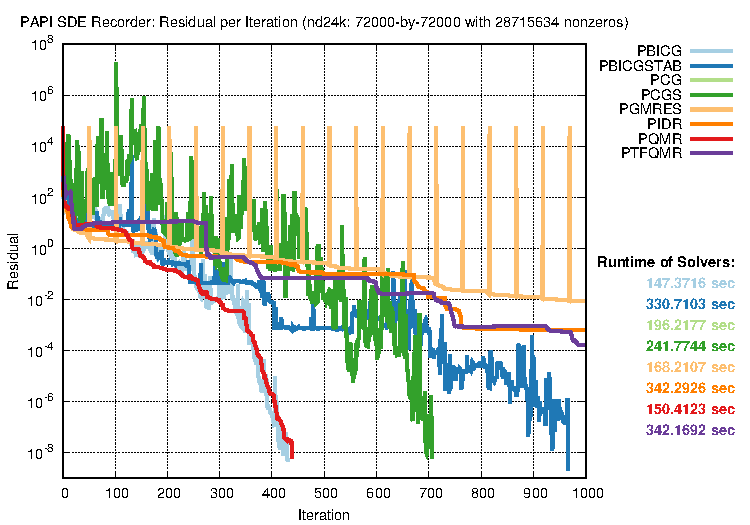
\includegraphics[width=0.49\linewidth]{projects/2.3.2-Tools/2.3.2.06-EXA-PAPI/Exa-PAPI_sde_magma.pdf}}
  \subfloat[ ]{\label{fig:sde_parsec}
  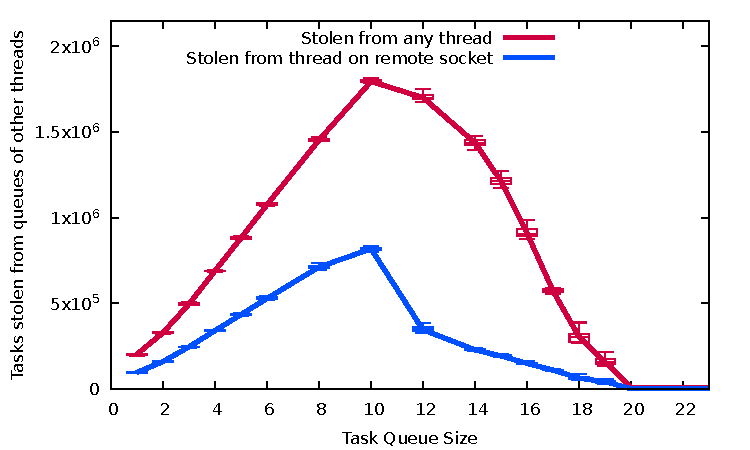
\includegraphics[width=0.49\linewidth]{projects/2.3.2-Tools/2.3.2.06-EXA-PAPI/Exa-PAPI_sde_parsec.pdf}}
\caption{(a) PAPI SDE-Recorder logging convergence of different ILU-preconditioned MAGMA-sparse Krylov solvers for a 2D/3D Problem; (b) PAPI SDE-Recorder logging the status of different task queues in PaRSEC.}
\end{center}
\end{figure}
\vspace{-8pt}
%
%
The examples in Figure~\ref{fig:sde_magma} illustrate how the convergence of Krylov solvers can be
visualized with the help of PAPI SDEs. Each of these solvers behave very differently 
for different problems and matrices, which, once more, stresses the importance of 
\emph{exposing these details in a standardized way}. This allows the domain
scientist to quickly identify the fastest and most robust method of choice for 
their very unique problems. Most importantly, this information can now be obtained without 
expert knowledge about algorithm-specific characteristics,
and without having to instrument MAGMA library code, but simply by calling \verb+PAPI_read()+
in the top-level application.

Figure~\ref{fig:sde_parsec} serves as a second showcase, illustrating the evolution of 
various task queues during the execution of a Cholesky factorization in PaRSEC.
With SDEs in PARSEC, a user can get a view of what is happening inside the runtime
by simply calling \verb+PAPI_start()+ and \verb+PAPI_stop()+ in their application, without the need to
instrument the PaRSEC runtime code. 



\vspace{10pt}
On the \textbf{hardware counter} front, we have developed a new PAPI component, called ``PCP'' for 
IBM Power9 hardware counters. It adds support for (1) core performance events, which are specific
to each core; and (2) shared events, which monitor the performance of
node-wide resources that are shared between cores. Access to shared
events require elevated privileges. However, IBM's official route for providing
access to shared events is through the Performance Co-Pilot (PCP) for non-root users.
The new PAPI-PCP component---available from the PAPI git repository (https://bitbucket.org/icl/papi.git)---enables 
all users to access Power9 shared events through PAPI.
(A report is publicly available on Jira:
\url{https://jira.exascaleproject.org/secure/attachment/13461/2018-06__Exa-PAPI__PCP__Milestone_Report.pdf})

\paragraph{Next Steps}

Our next efforts will focus on:
\begin{enumerate}
\item \textbf{PAPI Support for NVIDIA GPU Next-generation Monitoring Capabilities:} 
		Develop support for NVIDIA GPU performance counters and power 
		monitoring and capping capabilities. The released version of PAPI 
		will have fully integrated support for the NVIDIA GPU counters and power management.
%
\item \textbf{Prototype Tool to Assist with Native Counter Disambiguation}: 
		Create a prototype toolkit consisting of a collection of benchmarks 
		(some implemented as part of Exa-PAPI; some collected from existing 
		benchmark suites) that can assist developers in understanding the differences 
		between different native hardware events.
%
\item \textbf{Fulfillment of Software-defined Event Implementation}:
		Refine the PAPI component for SDEs based on feedback from the ECP community 
		and experience acquired from instrumenting ECP projects.
\end{enumerate}
